%%%%%%%%%%%%%%%%%%%%%%%%%%%%%%%%%%%%%%%%%%%%%%%%%%%%%%%%%%%%%
%% Begin exercise %%
%%%%%%%%%%%%%%%%%%%%%%%%%%%%%%%%%%%%%%%%%%%%%%%%%%%%%%%%%%%%%
\ex{Modelling and control: transfer functions, compensator and delay}

%%%%%%%%%%%%%%%%%%%%%%%%%%%%%%%%%%%%%%%%%%%%%%%%%%%%%%%%%%%%%
%% Task 1 %%
%%%%%%%%%%%%%%%%%%%%%%%%%%%%%%%%%%%%%%%%%%%%%%%%%%%%%%%%%%%%%

\task{Transfer functions of the buck}

A buck converter (brief B1 operating point, hard-switched for this task) converts \SI{48}{\volt} to \SI{12}{\volt} at \SI{100}{\watt} ($R=\SI{1.44}{\ohm}$) and $f_\mathrm{sw}=\SI{1}{\mega\hertz}$ with $L=\SI{2.2}{\micro\henry}$ and $C=\SI{20}{\micro\farad}$ ($R_\mathrm{esr}=\SI{2}{\milli\ohm}$). The PWM ramp has $V_\mathrm{M}=\SI{1}{\volt}$, the sensor $H=1$ (Fig.~\ref{fig:ex12_loop}).

%%%%%%%%%%%%%%%%%%%%%%%%%%%%%%%%%%%%%%%%%%%%%%%%%%%%%%%%%%%%%%%%%%%%%%%%%%
% Voltage-mode control loop (Exercise 12, Tasks 1 to 3)
%%%%%%%%%%%%%%%%%%%%%%%%%%%%%%%%%%%%%%%%%%%%%%%%%%%%%%%%%%%%%%%%%%%%%%%%%%

\begin{figure}[htb]
	\begin{center}
		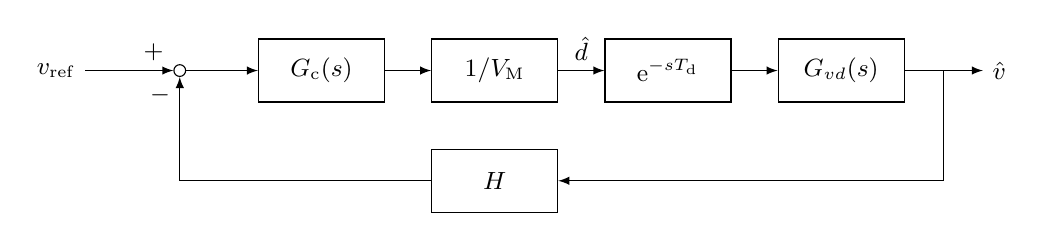
\begin{tikzpicture}[font=\small, >=latex, box/.style={draw, minimum width=1.6cm, minimum height=0.8cm, align=center}]
			\node[draw, circle, inner sep=1.5pt] (sum) at (0,0) {};
			\node[box] (gc) at (1.8,0) {$G_\mathrm{c}(s)$};
			\node[box] (pwm) at (4.0,0) {$1/V_\mathrm{M}$};
			\node[box] (del) at (6.2,0) {$\mathrm{e}^{-sT_\mathrm{d}}$};
			\node[box] (gvd) at (8.4,0) {$G_{vd}(s)$};
			\node[box] (h) at (4.0,-1.4) {$H$};
			\draw[->] (-1.2,0) node[left]{$v_\mathrm{ref}$} -- (sum.west) node[above left]{$+$};
			\draw[->] (sum) -- (gc); \draw[->] (gc) -- (pwm); \draw[->] (pwm) -- node[above]{$\hat{d}$} (del); \draw[->] (del) -- (gvd);
			\draw[->] (gvd) -- (10.2,0) node[right]{$\hat{v}$};
			\draw[->] (9.7,0) |- (h.east); \draw[->] (h.west) -| (sum.south) node[below left]{$-$};
		\end{tikzpicture}
	\end{center}
	\caption{Voltage-mode loop with modulator gain $1/V_\mathrm{M}$, total delay $T_\mathrm{d}$ and sensor gain $H$; loop gain $T=HG_\mathrm{c}G_{vd}\mathrm{e}^{-sT_\mathrm{d}}/V_\mathrm{M}$}
	\label{fig:ex12_loop}
\end{figure}


\subtask{Calculate $f_0$, $Q$, the characteristic impedance $Z_0=\sqrt{L/C}$, the ESR zero and the peak of $|G_{vd}|$. Why is the peak about $Q$ times the low-frequency gain?}

\begin{solutionblock}
	$f_0=1/(2\pi\sqrt{LC})=\SI{24.0}{\kilo\hertz}$, $Q=R\sqrt{C/L}=4.34$, $Z_0=\SI{332}{\milli\ohm}$, $f_\mathrm{esr}=1/(2\pi R_\mathrm{esr}C)=\SI{3.98}{\mega\hertz}$. $G_{vd}(0)=V_\mathrm{in}=\SI{48}{\volt}$ (\SI{33.6}{dB}); at $f_0$ the denominator reduces to $\mathrm{j}/Q$: $|G_{vd}|\approx QV_\mathrm{in}=208$ (\SI{46.4}{dB}); the exact value with ESR is 203. The $LC$ filter is lightly damped by the load.
\end{solutionblock}

\subtask{Show that the open-loop output impedance equals $R$ at $f_0$ (neglect ESR). What does this mean for a load step?}

\begin{solutionblock}
	$Z_\mathrm{out}=sL\,\|\,(1/sC)\,\|\,R$; at $\omega_0$ the parallel $LC$ is an open circuit, so $Z_\mathrm{out}=R=\SI{1.44}{\ohm}$ (\SI{1.40}{\ohm} with ESR), compared with $Z_0=\SI{0.33}{\ohm}$ for a well-damped filter. Without feedback a load step excites a ringing at \SI{24}{\kilo\hertz}; the averaged model gives \SI{2.2}{\volt} peak for an \SI{8}{\ampere} step.
\end{solutionblock}

\subtask{A boost converter (12 to \SI{48}{\volt}, \SI{100}{\watt}, $L=\SI{4.7}{\micro\henry}$) has a right-half-plane zero. Where is it, and what limits the crossover frequency?}

\begin{solutionblock}
	$D'=0.25$, $R=\SI{23}{\ohm}$: $f_\mathrm{z}=D'^2R/(2\pi L)=\SI{48.8}{\kilo\hertz}$. The crossover must stay well below, at about \SI{10}{\kilo\hertz}, independent of $f_\mathrm{sw}$.
\end{solutionblock}

%%%%%%%%%%%%%%%%%%%%%%%%%%%%%%%%%%%%%%%%%%%%%%%%%%%%%%%%%%%%%
%% Task 2 %%
%%%%%%%%%%%%%%%%%%%%%%%%%%%%%%%%%%%%%%%%%%%%%%%%%%%%%%%%%%%%%

\task{Type III compensator}

\begin{equation}
	G_\mathrm{c}(s)=\frac{\omega_\mathrm{I}}{s}\,\frac{(1+s/\omega_\mathrm{z})^2}{(1+s/\omega_\mathrm{p})^2}
\end{equation}

\subtask{Place the zeros at $0.8f_0$ and the poles at $f_\mathrm{sw}/2$ and determine $\omega_\mathrm{I}$ for $f_\mathrm{c}=\SI{100}{\kilo\hertz}$. Calculate the phase margin (notebook).}

\begin{solutionblock}
	$f_\mathrm{z}=\SI{19.2}{\kilo\hertz}$, $f_\mathrm{p}=\SI{500}{\kilo\hertz}$; $|T(\mathrm{j}2\pi\cdot\SI{100}{\kilo\hertz})|=1$ gives $\omega_\mathrm{I}=\SI{7.9\cdot10^{3}}{\per\second}$ (integrator unity-gain frequency \SI{1.26}{\kilo\hertz}). Phase margin \ang{50.5}.
\end{solutionblock}

\subtask{Estimate the output deviation for an \SI{8}{\ampere} load step with $\Delta v\approx\Delta I/(2\pi f_\mathrm{c}C)$ and compare with the averaged closed-loop model. Which crossover would limit the deviation to \SI{0.3}{\volt}?}

\begin{solutionblock}
	Estimate \SI{0.64}{\volt}; the closed-loop output impedance $Z_\mathrm{out}/(1+T)$ gives \SI{0.52}{\volt} after \SI{2.3}{\micro\second} (open loop \SI{2.2}{\volt}). For \SI{0.3}{\volt}: $f_\mathrm{c}=\SI{212}{\kilo\hertz}\approx f_\mathrm{sw}/5$, at the limit for PWM control. More output capacitance, current-mode or ripple-based control are the alternatives.
\end{solutionblock}

%%%%%%%%%%%%%%%%%%%%%%%%%%%%%%%%%%%%%%%%%%%%%%%%%%%%%%%%%%%%%
%% Task 3 %%
%%%%%%%%%%%%%%%%%%%%%%%%%%%%%%%%%%%%%%%%%%%%%%%%%%%%%%%%%%%%%

\task{Loop delay}

\subtask{A digital controller adds $T_\mathrm{d}=1.5\,T_\mathrm{s}$. Calculate the phase lag at \SI{100}{\kilo\hertz} and the remaining margin. Which total delay still leaves \ang{30}?}

\begin{solutionblock}
	$360^\circ\cdot\SI{100}{\kilo\hertz}\cdot\SI{1.5}{\micro\second}=\ang{54}$: margin $\ang{50.5}-\ang{54}=\ang{-3.5}$, unstable. For \ang{30} the delay may cost \ang{20.5}: $T_\mathrm{d}\leq\SI{0.57}{\micro\second}=0.57\,T_\mathrm{s}$, e.g.\ sampling synchronised with the PWM and a computation within half a period.
\end{solutionblock}

\subtask{Can the margin be restored by reducing $\omega_\mathrm{I}$ only (lower crossover)? Explain with the phase of the loop below \SI{100}{\kilo\hertz} (notebook).}

\begin{solutionblock}
	No. Between 30 and \SI{100}{\kilo\hertz} the margin with delay stays below \ang{30} (\ang{28} at \SI{31}{\kilo\hertz}, \ang{16} at \SI{60}{\kilo\hertz}): close to $f_0$ the $LC$ double pole has turned the phase by almost \ang{180}, and the compensator zeros at \SI{19}{\kilo\hertz} have not yet recovered it. A voltage-mode loop with such a delay must cross well below $f_0$, i.e.\ become slow, unless the delay is reduced or an inner current loop removes the double pole.
\end{solutionblock}

%%%%%%%%%%%%%%%%%%%%%%%%%%%%%%%%%%%%%%%%%%%%%%%%%%%%%%%%%%%%%
%% Task 4 %%
%%%%%%%%%%%%%%%%%%%%%%%%%%%%%%%%%%%%%%%%%%%%%%%%%%%%%%%%%%%%%

\task{Current-mode and ripple-based control}

\subtask{Peak current mode, buck 12 to \SI{7.2}{\volt}, $L=\SI{2.2}{\micro\henry}$, \SI{1}{\mega\hertz}. Calculate $m_1$, $m_2$, the factor of a valley-current perturbation and Ridley's $Q_\mathrm{p}$ for $m_\mathrm{a}=0$, $m_2/2$ and $m_2$. Simulate the inductor current for a perturbation of \SI{0.15}{\ampere} (notebook).}

\begin{solutionblock}
	$m_1=(12-7.2)\,\mathrm{V}/\SI{2.2}{\micro\henry}=\SI{2.18}{\ampere\per\micro\second}$, $m_2=\SI{3.27}{\ampere\per\micro\second}$, $D=0.6$.
	$m_\mathrm{a}=0$: factor $-1.5$, unstable ($Q_\mathrm{p}\to\infty$). $m_\mathrm{a}=m_2/2$: $-0.43$, $m_\mathrm{c}=1.75$, $Q_\mathrm{p}=1/(\pi(m_\mathrm{c}D'-0.5))=1.59$. $m_\mathrm{a}=m_2$: factor 0 (a perturbation vanishes in one period), $Q_\mathrm{p}=0.64$; more ramp makes the loop behave more like voltage mode.
\end{solutionblock}

\subtask{A constant-on-time buck uses $t_\mathrm{on}=\SI{250}{\nano\second}$ for 48 to \SI{12}{\volt}. Calculate $f_\mathrm{sw}$ at 36, 48 and \SI{60}{\volt}. How is the frequency kept constant?}

\begin{solutionblock}
	$f_\mathrm{sw}=V_\mathrm{out}/(V_\mathrm{in}t_\mathrm{on})$: \SI{1.33}{\mega\hertz}, \SI{1.00}{\mega\hertz}, \SI{0.80}{\mega\hertz}. With $t_\mathrm{on}=V_\mathrm{out}/(V_\mathrm{in}f_\mathrm{set})$, generated from the input and output voltages, the frequency stays near \SI{1}{\mega\hertz}; losses and dead times still shift it slightly, and the load transient changes it temporarily.
\end{solutionblock}

%%%%%%%%%%%%%%%%%%%%%%%%%%%%%%%%%%%%%%%%%%%%%%%%%%%%%%%%%%%%%
%% Task 5 %%
%%%%%%%%%%%%%%%%%%%%%%%%%%%%%%%%%%%%%%%%%%%%%%%%%%%%%%%%%%%%%

\task{Control concept of your brief (homework, milestone M3)}

\subtask{Choose the control method of your converter and justify it with numbers: control input, crossover, margins, delays of driver, comparator or digital controller, and the operating range (ZVS boundary, RHP zero, gain curve).}

\begin{solutionblock}
	Check list: averaged or envelope model of the plant at the worst-case operating points; loop gain with all delays; margins over the input and load range; behaviour at start-up and light load (burst, DCM); measurement of the loop gain on the hardware.
\end{solutionblock}

\vspace{0.5cm}
Remark: The notebook \texttt{tutorialEx12\_task.ipynb} builds the averaged buck model, designs the compensator, evaluates the delay, simulates current-mode control with slope compensation and computes the constant-on-time frequency.
